\subsection{Transformada de Fourier Discreta 2D}

\begin{frame}
\frametitle{Introducci\'{o}n Transformada de Fourier 2D}

\small

En el caso de las se\~{n}ales 1D (que hemos representado habitualmente frente al tiempo) hemos visto 3 Transformadas de Fourier diferentes:
\begin{itemize}

\item Transformada de Fourier continua ($x(t) \rightarrow X(jw)$). Se utiliza para se\~{n}ales continuas y obtiene transformadas en frecuencias continuas

\item Transformada de Fourier en tiempo discreto ($x(n) \rightarrow X(e^{jw})$). Se utiliza para se\~{n}ales discretas y obtiene transformadas en frecuencias continuas.

\item Transformada de Fourier discreta (FFT, $x(n) \rightarrow X(k)$). Se utiliza para se\~{n}ales discretas y obtiene transformadas en frecuencias discretas.

\end{itemize}

\visible<2->{
Como la \'{u}ltima es la que se puede computar facilmente con un ordenador y se relaciona con las anteriores (represent\'{a}ndola ante $w_d=2 \pi*[0:N-1]/N$ \'{o} $w_c=w_d*F_s$), vamos a ver directamente la
Transformada de Fourier Discreta (FFT) para im\'{a}genes digitales. }

\vspace{0.1cm}

\visible<3->{
Antes de proceder, hay que tener en cuenta que:

\vspace{-0.7cm}

\begin{columns}[t]

\begin{column}{6cm}

\begin{itemize}
\item $u=sen(w_c*t)$ y  $w_c=\frac{2\pi}{T}$ rad/s

\vspace{-0.2cm}

\item $u=sen(w_c*x)$ y $w_c= \frac{2\pi}{T}$ rad/m
\end{itemize}

\end{column}

\visible<4->{
\begin{column}{3cm}

\begin{itemize}


\item $t=n \cdot T_s$

\vspace{-0.2cm}

\item $x= n \cdot D_x$\end{itemize}

\end{column}}


\end{columns}

}

\end{frame}


\begin{frame}
\frametitle{Definici\'{o}n de la Transformada de Fourier Discreta 2D }

\small

Definiciones para se\~{n}ales 1D f(n) de longitud N:

\vspace{0.1cm}


\begin{itemize}

\item  $X(k)=DFT(x(n))=\sum_{n=0}^{N-1} x(n) e^{- j \frac{2 \pi  k}{N} n}=\sum_{n=0}^{N-1} x(n) e^{-2\pi j \frac{ kn}{N}}$


\visible<3->{
\vspace{0.2cm}

\item  $x(n)=IDFT(X(k))=\frac{1}{N} \sum_{k=0}^{N-1} X(k) e^{2\pi j \frac{ kn}{N}}$}

\end{itemize}

\vspace{0.2cm}

\hrule

\vspace{0.2cm}


\small

\visible<2->{
Definiciones para se\~{n}ales 2D f(m,n) de tama\~{n}o $M x N$):

\vspace{0.1cm}

\begin{itemize}

\item $F(u,v)=DFT(f(m,n))= \sum_{m=0}^{M-1} \sum_{n=0}^{N-1} f(m,n) e^{-2\pi j (\frac{mu}{M}+\frac{nv}{N})}$

\visible<4->{

\vspace{0.2cm}

\item $f(m,n)=IDFT(f(u,v))=\frac{1}{NM} \sum_{u=0}^{M-1} \sum_{v=0}^{N-1} F(u,v) e^{ 2\pi j (\frac{mu}{M}+\frac{nv}{N})}$}

\vspace{0.2cm}

\visible<5->{
\item En el caso de ser una imagen de tama\~{n}o $M*M$ podemos darle 1/M a la DFT y 1/M a la IDFT.

}

\end{itemize}
}



\visible<6->{
\vspace{0.2cm}

Computo de la DFT de imagen con Matlab: \color{blue}IM=fft2(im)\color{black}}


\end{frame}

%%%%%%%%%%%%
%%%%%%%%%%%%

\begin{frame}
\frametitle{Ejemplos de Transformada de Fourier Discreta 2D}

\small

\color{olivegreen} Ejemplo: \color{black} DFT de una se\~{n}al 1D

\begin{columns}[t]

\begin{column}{3.8cm}

\vspace{-0.7cm}


\lstinputlisting{./Matlab/TransformadaDiscreta1_1D.m}


\end{column}

\hspace{-0.3cm}\begin{column}{3.5cm}

\includegraphics[width=3.5cm,trim={0cm 0cm 0cm 0cm},clip,angle=0]{./Figures/D1_Tiempo.eps}

\end{column}

\hspace{-0.4cm}\begin{column}{3.5cm}

\includegraphics[width=3.5cm,trim={0cm 0cm 0cm 0cm},clip,angle=0]{./Figures/D1_DFT.eps}

\end{column}


\end{columns}

%%%%%%%%%%%%%%%%%%%%%

\visible<2->{


\color{olivegreen} Ejemplo: \color{black} DFT de una se\~{n}al 2D

\begin{columns}[t]

\begin{column}{4.2cm}

\vspace{-0.7cm}


\lstinputlisting{./Matlab/TransformadaDiscreta1_2D.m}


\end{column}

\hspace{-0.3cm}\begin{column}{3.5cm}


\includegraphics[width=3.5cm,trim={0cm 0cm 0cm 0cm},clip,angle=0]{./Figures/D2_Tiempo.eps}

\end{column}

\hspace{-0.4cm}\begin{column}{3.5cm}

\includegraphics[width=3.5cm,trim={0cm 0cm 0cm 0cm},clip,angle=0]{./Figures/D2_DFT.eps}

\end{column}


\end{columns}


}

\end{frame}



%%%%%%%%%%%%
%%%%%%%%%%%%


\begin{frame}
\frametitle{Ejemplos de Transformada de Fourier Discreta 2D}

\small

\color{olivegreen} Ejemplo: \color{black} DFT de una se\~{n}al 1D (con fftshift)

\begin{columns}[t]

\begin{column}{3.8cm}

\vspace{-0.7cm}


\lstinputlisting{./Matlab/TransformadaDiscreta2_1D.m}


\end{column}

\hspace{-0.3cm}\begin{column}{3.5cm}

\includegraphics[width=3.5cm,trim={0cm 0cm 0cm 0cm},clip,angle=0]{./Figures/D1_DFT.eps}

\end{column}

\hspace{-0.4cm}\begin{column}{3.5cm}

\includegraphics[width=3.5cm,trim={0cm 0cm 0cm 0cm},clip,angle=0]{./Figures/D1_DFT2.eps}

\end{column}


\end{columns}

%%%%%%%%%%%%%%%%%%%%%

\visible<2->{


\color{olivegreen} Ejemplo: \color{black} DFT de una se\~{n}al 2D (con fftshift)

\begin{columns}[t]

\begin{column}{4.2cm}

\vspace{-0.7cm}


\lstinputlisting{./Matlab/TransformadaDiscreta2_2D.m}


\end{column}

\hspace{-0.3cm}\begin{column}{3.5cm}

\includegraphics[width=3.5cm,trim={0cm 0cm 0cm 0cm},clip,angle=0]{./Figures/D2_DFT.eps}

\end{column}

\hspace{-0.4cm}\begin{column}{3.5cm}

\includegraphics[width=3.5cm,trim={0cm 0cm 0cm 0cm},clip,angle=0]{./Figures/D2_DFT2.eps}

\end{column}


\end{columns}


}

\end{frame}



%%%%%%%%%%%%
%%%%%%%%%%%%

\begin{frame}
\frametitle{Ejemplos de Transformada de Fourier Discreta 2D}

\small

\color{olivegreen} Ejemplo: \color{black} DFT de se\~{n}ales 2D con distinta orientacion
\begin{columns}[t]

\begin{column}{3.8cm}

\vspace{-0.5cm}


\lstinputlisting{./Matlab/TransformadaDiscreta3_2D.m}


\end{column}

\hspace{-0.3cm}\begin{column}{2cm}

\includegraphics[width=1.7cm,trim={0cm 0cm 0cm 0cm},clip,angle=0]{./Figures/ROT_IM0.eps}


\includegraphics[width=1.7cm,trim={0cm 0cm 0cm
0cm},clip,angle=0]{./Figures/ROT_DFD0.eps}

\scriptsize

\color{gray} angle=0

\end{column}


\hspace{-0.3cm}\begin{column}{2cm}


\includegraphics[width=1.7cm,trim={0cm 0cm 0cm 0cm},clip,angle=0]{./Figures/ROT_IM45.eps}


\includegraphics[width=1.7cm,trim={0cm 0cm 0cm
0cm},clip,angle=0]{./Figures/ROT_DFD45.eps}

\scriptsize

\color{gray} angle=45

\end{column}


\hspace{-0.3cm}\begin{column}{2cm}


\includegraphics[width=1.7cm,trim={0cm 0cm 0cm 0cm},clip,angle=0]{./Figures/ROT_IM90.eps}

\includegraphics[width=1.7cm,trim={0cm 0cm 0cm
0cm},clip,angle=0]{./Figures/ROT_DFD90.eps}

\scriptsize

\color{gray} angle=90

\end{column}


\end{columns}

%%%%%%%%%%%%%%%%%%%%%

\visible<2->{


\color{olivegreen} Ejemplo: \color{black} DFT de una se\~{n}al 2D real (re-escalado de la DFT)

\begin{columns}[t]

\begin{column}{4.2cm}

\vspace{-0.7cm}


\lstinputlisting{./Matlab/TransformadaDiscreta4_2D.m}




\end{column}

\hspace{-0.3cm}\begin{column}{2cm}


\includegraphics[width=2cm,trim={0cm 0cm 0cm 0cm},clip,angle=0]{./Figures/estanteria_1.eps}

\end{column}

\hspace{-0.4cm}\begin{column}{2cm}


\includegraphics[width=2cm,trim={0cm 0cm 0cm 0cm},clip,angle=0]{./Figures/estanteria_2.eps}
\end{column}

\hspace{-0.4cm}\begin{column}{2cm}

\includegraphics[width=2cm,trim={0cm 0cm 0cm 0cm},clip,angle=0]{./Figures/estanteria_3.eps}
\end{column}


\end{columns}

\footnotesize
\color{red}  Reescalar: $log_{10}(1+|F(u,v)|^2)$


}

\end{frame}

%%%%%%%%%%%%%%%%%%%%%%%%

\begin{frame}
\frametitle{Propiedades de la DFT 2D}

\footnotesize

 \hspace{0.4cm} $F(u,v)=DFT(f(m,n))=\frac{1}{NM} \sum_{m=0}^{M-1} \sum_{n=0}^{N-1} f(m,n) e^{-2\pi j (\frac{mu}{M}+\frac{nv}{N})}$

 \vspace{0.2cm}

La DFT tiene las siguientes propiedades:

\begin{itemize}

\item \alert{\textit{Separabilidad}}: como $e^{-2\pi j (\frac{mu}{M}+\frac{nv}{N})}=e^{-2\pi j \frac{mu}{M}} e^{-2\pi j \frac{nv}{N}}$, la DFT se puede calcular $F(u,v)= \frac{1}{M} \sum_{m=0}^{M-1}\left[\frac{1}{N} \sum_{n=0}^{N-1} f(m,n) e^{-2\pi j \frac{nv}{N}} \right ] e^{-2\pi j \frac{mu}{M}}$, es decir a partir de la DFT 1D por filas y columnas.

\item  \alert{\textit{C\'{a}lculo matricial:}} (semejante a la DFT 1D)

\item  \alert{\textit{Traslaci\'{o}n}: }$ DFT(f(m-m_0,n-n_0))= e^{-j2 \pi (u \cdot m_0+v \cdot n_0)}F(u,v)$

\item \alert{\textit{Periodicidad}: } $F(u,v)=F(u+M,v)\!=\!F(u,v+N)\!=\!F(u+M,v+N)$

La DFT tienen un periodo de M y N

\item \alert{\textit{Simetr\'{i}a}} (si f(m,n) es real):  F(u,v)=F*(-u,-v) y  $|F(u,v)|=|F(-u,-v)|$

\item \alert{\textit{Rotaci\'{o}n:}} Si rotamos una imagen $\theta$ grados, tambi\'{e}n rotamos la DFT los mismos grados.

\item \alert{\textit{Linealidad}}

\item \alert{\textit{Escalado:}} $DFT(f(am,bn)=\frac{1}{ab}F(u/a,v/b)$


\end{itemize}


\hrule

\vspace{0.2cm}

\scriptsize
\color{gray} Las propiedades de periodicidad y simetr\'{i}a son las que nos permiten hacer el fftshift.

\end{frame}
